\documentclass{ximera}
%%\colorlet{penColor}{blue!50!black} % Color of a curve in a plot
%\colorlet{gridColor}{gray!50} % Color of grid in a plot
%\colorlet{background}{white} % Color of the page
\newcommand{\ddx}{\frac{d}{dx}}
\newcommand{\dydx}{\frac{dy}{dx}}
\newcommand{\dd}[2][]{\frac{d #1}{d #2}}


\outcome{Understand a function as a transformation of its input into its output.}

\outcome{Understand that for every value in the domain, there is exactly one value in the range.}

\outcome{Understand when a function is invertible.}

\outcome{Interpret a function from an algebraic, numerical, graphical
  and verbal perspective.}

\title{Review of functions}

\begin{document}

\begin{abstract}
  This activity will get you thinking about some concepts related to
  functions that are relevant to calculus.
\end{abstract}
\maketitle


\begin{question}
  A number $x$, is to a function $f$, is to a number $f(x)=y$ as:
  %% Alternatively we could use: An angle, is to $\sin$, is to a length as:
  \begin{hint}
      The notation for functions can be confusing. The letter $f$ is
      the ``name'' of the function. Technically, $f(x)$ is the output;
      however, to remind students that $f$ is in fact a function, it
      is common to call the function $f(x)$. For more on this,
      see\link{http://www.purplemath.com/modules/fcnnot.htm}
  \end{hint}
  \begin{hint}
    If you are confused, see\href{http://en.wikipedia.org/wiki/Function_(mathematics)}{This link}.
  \end{hint}
  \begin{multipleChoice}
    \choice[correct]{URL, is to a web browser, is to web page.}
    \choice{URL, is to web page, is to a web browser.}
    \choice{Web page, is to a web browser, is to URL.}
    \choice{Web page, is to URL, is to a web browser.}
    \choice{A web browser, is to web page, is to URL.}
    \choice{A web browser, is to URL, is to web page.}
  \end{multipleChoice}
\end{question}


\begin{question}
  On which interval(s) is the function depicted below invertible?
  \begin{image}
    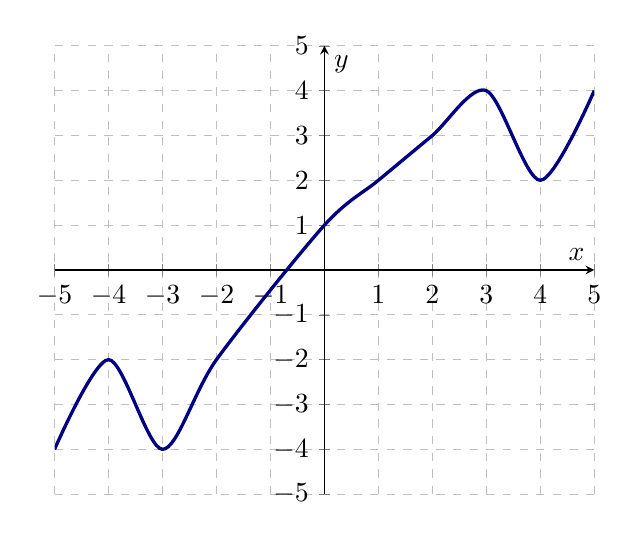
\begin{tikzpicture}
        \begin{axis}[
            xmin=-5,
            xmax=5,
            ymin=-5,
            ymax=5,
            axis lines =middle,
            every axis y label/.style={at=(current axis.above origin),anchor=south},
            every axis x label/.style={at=(current axis.right of origin),anchor=west},
            axis lines =middle, xlabel=$x$, ylabel=$y$,
            xtick={-5,-4,...,5},
            ytick={-5,-4,...,5},
            grid=both,
            grid style={dashed, gray!50},
          ]
          ]
          \addplot [very thick, blue!50!black, smooth] coordinates {
            (-5,-4)
            (-4,-2)
            (-3,-4)
            (-2,-2)
            (-1.-1)
            (0,1)
            (1,2)
            (2,3)
            (3,4)
            (4,2)
            (5,4)
          };
        \end{axis}
    \end{tikzpicture}
  \end{image}
  \begin{hint}
    If you are confused,
    see\link{http://en.wikipedia.org/wiki/Inverse_function#Graph_of_the_inverse}.
  \end{hint}
  \begin{multipleChoice}
      \choice[correct]{$-2<x<1$}
      \choice{$-3<x<3$}
      \choice{$-4<x<4$}
      \choice{$-3<x<4$}
      \choice{$-4<x<3$}
      \choice{$-5<x<-4$ and $-3<x<3$ and $4<x<5$}
      \choice{$-4<x<-3$ and $3<x<4$}
      \choice{For all real values of $x$}
      \choice{For no real values of $x$}
    \end{multipleChoice}  
\end{question}


\begin{question}
  Which of the following statements is true?
  %% Alternatively we could use $\sqrt{x}$
  \begin{hint}
    If you are confused, see\link{http://en.wikipedia.org/wiki/Inverse_trigonometric_functions}.
  \end{hint}
  \begin{multipleChoice}
    \choice[correct]{$\sin\left(\sin^{-1}\left(\frac{1}{2}\right)\right)
      = \frac{1}{2}$} 
    \choice{$\sin^{-1}\left(\sin\left(\frac{5\pi}{2}\right)\right) = \frac{5\pi}{2}$}
    \choice{$\sin^{-1}(x)$ is the inverse function of $\sin(x)$}
    \choice{$\sin^{-1}(x) = \frac{1}{\sin(x)}$}
  \end{multipleChoice}  
\end{question}



\begin{question}
  The expression $\log_b(x) = y$ is equivalent to:
  \begin{hint}
    If you are confused, see\link{http://en.wikipedia.org/wiki/Logarithm}.
  \end{hint}
  \begin{multipleChoice}
    \choice[correct]{$b^y = x$}
    \choice{$b^x = y$}
    \choice{$x^y = b$}
    \choice{$y^x = b$}
    \choice{$x^b = y$}
    \choice{$y^b = x$}
  \end{multipleChoice}  
\end{question}

\begin{question}
What other questions do you have about this lecture?
\begin{free-response}
  Answers will vary.
\end{free-response}
\end{question}

\end{document}
